\documentclass[a4paper,12pt]{article}

% Packages de base
\usepackage[utf8]{inputenc}
\usepackage[T1]{fontenc}
\usepackage[english,french]{babel}
\usepackage[margin=2.5cm]{geometry}

% Packages utiles
\usepackage{graphicx} % Pour les images
\usepackage{hyperref} % Liens cliquables
\usepackage{amsmath}  % Mathématiques avancées
\usepackage{enumitem} % Listes personnalisées
\usepackage{titling}  % Permet de mofif le title
\usepackage{float}    % Permet le positionnement des images
\usepackage{listings} % Permet les blocs de code avec coloration syntaxique
\usepackage{xcolor}   % Permet de mettre des paragraphes en couleur
\usepackage{amsfonts} % Permet d'avoir les ensembles mathématiques
\usepackage{minted}   % Bloc de codes propres 
\usepackage{stmaryrd} % Pour \llbracket et \rrbracket

% Options
\setcounter{tocdepth}{3}       % Inclure les sous-sections
\usepackage[none]{hyphenat}    % Evite les cesures dans tous le document
\usepackage[minted]{tcolorbox} % Config pour minted

% Définir des couleurs customs
\definecolor{darkgreen}{rgb}{0.0, 0.4, 0.0}           % Vert très foncé
\definecolor{cyan}{rgb}{0.0, 0.6, 0.8}                % Cyan
\definecolor{red}{rgb}{0.6, 0.0, 0.0}                 % Rouge très foncé
\definecolor{lightgray}{rgb}{0.95, 0.95, 0.95}        % Gris clair

\definecolor{monokai-bg}{HTML}{272822}                % BG pour monokai

% Style personnalisé pour les blocs de code
\newtcblisting{pythoncode}{
  listing engine=minted,
  colback=monokai-bg,
  colframe=black,
  listing only,
  minted style=monokai,
  minted language=python, % Changez ici pour un autre langage si besoin
  minted options={
    linenos,
    fontsize=\small,
    breaklines,
    escapeinside=||,
    tabsize=4
  },
  left=5pt,
  right=5pt,
  top=5pt,
  bottom=5pt,
  boxrule=0.5pt,
  arc=4pt
}

\newtcblisting{bashcode}{
  listing engine=minted,
  colback=lightgray,
  colframe=black,
  listing only,
  minted style=friendly,
  minted language=bash,
  minted options={
    linenos,
    fontsize=\small,
    breaklines,
    escapeinside=||,
    tabsize=4
  },
  left=5pt,
  right=5pt,
  top=5pt,
  bottom=5pt,
  boxrule=0.5pt,
  arc=4pt
}

% Premiere page
\title{Python pour les incultes}
\author{Bodin Jules}
\date{\today}

\renewcommand{\maketitlehookd}{%
    \begin{center}
    
\includegraphics[keepaspectratio=true, width=0.8\textwidth]{../images/Logo_Python.jpg}
    \end{center}
}

\begin{document}

% Page de titre
\maketitle

% Page d'introduction avant la table des matieres
% Expliques comment est design ce pdf
\newpage

Ce document a pour but d'enseigner les rudiments de Python. Python est muni d'une multitude de packages\footnote{Un package en Python, 
c’est juste un dossier qui contient plusieurs fichiers Python (appelés modules) et qui permet d’organiser le code. 
} qui ne sont pas à connaitre dans le cadre d'une CPGE (cf. \href{https://prepas.org/ups.php?rubrique=53}{prepas.org}). 
Cependant, un de ces packages est très utile dans un cadre d'analyse de données : \textbf{matplotlib} et sera surement utilisé en physique. 
Je recommande donc de s'y intéresser et une page à la fin de ce cours y sera dédiée pour aborder les bases de ce package 
(il est très conséquent).

Ce cours est construit pour être lu dans l'ordre des parties, mais il est aussi structuré pour permettre au lecteur de naviguer rapidement
et simplement dans ce dernier (car le temps c'est des places en prépa).
Il abordera toutes les notions nécessaires pour la prépa et plus encore, chaque point important étant accompagné d'un petit exemple. Attention cependant,
ces exemples ne suffiront pas à l'apprentissage de Python, seule la pratique régulière permettra de bien comprendre les notions abordées.

Pour finir, le programme d'informatique pour tous aborde les notions de complexité des algorithmes étudiés. Ce cours donnera les complexités associées en les 
justifiant mais les preuves ne seront pas données, le but étant ici de comprendre la notion de complexité plus que de savoir la démontrer
(les profs seront bien meilleurs à ce niveau).

Je rappelle qu'aucune matière ne doit être négligée en prépa, cependant il est plus intéressant d'insister sur celles ayant un plus gros coefficient. 
Ainsi, il est plus intelligent de bien gérer son temps (encore lui) et de ne pas chercher à maitriser parfaitement ce cours durant les 2 années de prépa. 
Comme le disait si bien mon professeur de physique de permière année : la progression dans une matière est similaire à celle d'un circuit RC,
plus tu y passes de temps et moins l'évolution est grande (Je précise que c'est dans le cas d'une charge hein).

\begin{figure}[H]
    \centering
    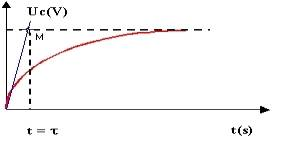
\includegraphics[keepaspectratio=true, width=0.8\textwidth]{../images/Charge_RC.jpg}
    \caption{Une charge de circuit RC au cas où le lecteur l'aurait oublié (pas bien ça)}
\end{figure}

\noindent Bonne lecture et bon courage, le chrono est déjà lancé.
\newpage

\tableofcontents % Table des matières optionnelle

\newpage

\section{Introduction}
Python est un des langages de programmation les plus utilisés.
C'est un langage de programmation interprété, multiparadigme et multiplateformes. Ses paradigmes sont : impératif, fonctionnel et orienté objet. 
Oui je sais, ça fait beaucoup de termes nouveaux pour un premier paragraphe d'introduction, mais il n'est pas nécessaire de tous les retenir tout de suite (c'est juste pour la culture).

On va se concentrer sur le terme le plus important : \underline{interprété}. En informatique, il existe deux catégories principales de langages : les compilés et les interprétés, auxquels s'ajoutent les hybrides (JIT, bytecode + VM, ...). Pour faire court, un langage compilé nécessite une étape de compilation qui traduit le code source en code machine (code illisible à l'oeil nu mais compréhensible par la machine) alors qu'un langage interprété lit le code source et l'exécute. Le premier est plus rapide à l'exécution car directement traduit pour la machine, le second est plus flexible et plus simple à apprendre. Nous allons le voir, Python fait beaucoup (voir \textbf{\underline{BEAUCOUP}}) de chose sans le montrer, dont une gestion automatique de la mémoire par ramasse-miettes. Pour finir, Python est doté d'un typage dynamique fort et d'un système de gestion d'exceptions.

\begin{figure}[h]
    \centering
    \begin{minipage}{0.45\textwidth}
        \centering
        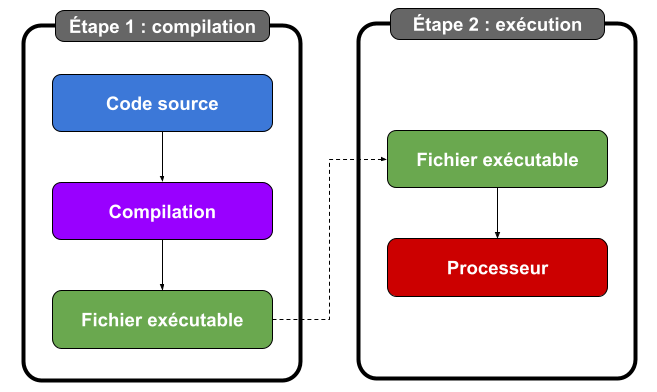
\includegraphics[height=4cm]{../images/compile.png}
        \caption{Langage compilé}
    \end{minipage}
    \hfill
    \begin{minipage}{0.45\textwidth}
        \centering
        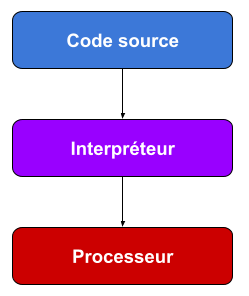
\includegraphics[height=4cm]{../images/interprete.png}
        \caption{Langage interprété}
    \end{minipage}
\end{figure}

Cool maintenant on sait qu'on va pas trop galérer à apprendre Python. Il est donc temps de s'y mettre.

\newpage

\section{Les bases}

On entre dans le vif du sujet, on va apprendre à coder en Python. 

\subsection{Création et Exécution}

Sous linux, pour créer un programme Python, il faut déjà créer le fichier qui va accueillir son code source. \newline
Pour cela, il suffit de se mettre dans le répertoire souhaité (avec $cd$ c'est mieux et ça fait plus pro) et de créer un fichier avec une extension ".py".
Voila la commande à entrer si on veut créer un programme nommé toto :

\begin{bashcode}
    touch toto.py
\end{bashcode}

{\color{darkgreen}
\noindent\textbf{Mini Exercice 2.1 : } Créer un programme tata.py dans un sous répertoire "Tutu/". \newline
\textit{Indication : } Regarder la commande mkdir \newline
Correction \hyperlink{AncreExo2.1}{ici}.\newline
}

On sait maintenant créer le fichier qui va accueillir le code source de notre programme. Cependant, il ne faut pas oublier que python est un langage \underline{interprété}.
Cela signifie qu'un fichier *.py n'est en fait qu'un fichier comprenant pleins de mots qui se suivent. Il faut que l'on indique à notre machine comment lire ce fichier.
Pour cela il existe 2 méthodes : 
\begin{itemize}
    \item \underline{Le Shebang :} Cette méthode consiste à ajouter une en-tête à notre fichier. Il faut écrire sur la \textbf{première} ligne. 
        \begin{pythoncode}
    #! /usr/bin/env python3
        \end{pythoncode}
        Qu'est ce que ce Shebang fait ? Il indique au système en quelle langue est écrit ce code source. Ici on lui indique que c'est en Python version 3.x. 
        Deux choses à noter cependant : 
        \begin{enumerate}
            \item Cette méthode ne fonctionne que sur système Unix
            \item On peut seulement écrire python au lieu de python3 sur le Shebang, cependant si plusieurs versions de python sont installées sur votre ordinateur, on en sait pas vers quoi pointera le Shebang.
        \end{enumerate}
        Avec cette méthode, il ne reste plus qu'à entrer le chemin vers le fichier dans le terminal pour l'exécuter.
    \item \underline{A la main :} Cette méthode consiste à préciser directement dans le terminal \\
        l'interpréteur à utiliser. Ce qui donne dans le terminal :
        \begin{bashcode}
    python3 /chemin/vers/le/fichier.py
        \end{bashcode}
\end{itemize}

\subsection{Hello world}

Le programme le plus classique à faire en informatique est celui qui affiche hello world dans le terminal. Il est grand temps que vous vous lanciez, mais je ne vais pas vous jetez dans la jungle sans rien.
En Python, la fonction qui permet d'afficher quelque chose dans le terminal est la fonction {\color{blue} print(*objects)}. 
Cette fonction est beaucoup plus complexe qu'elle ne le laisse paraitre, mais nous verrons ça plus tard. Tout ce que vous devez retenir c'est que print affiche ce que vous mettez dans le champ *objects.
De plus, en Python, le texte se met entre guillemets.

{\color{darkgreen}
\noindent\textbf{Mini Exercice 2.2 : } Créer un programme hello.py qui affiche "Hello World !" dans le terminal. \newline
\textit{Indication : } Sans compter le Shebang, ce programme tiens sur une seule ligne ! \newline
Correction \hyperlink{AncreExo2.2}{ici}.\newline
}

Félicitation, vous venez de faire votre baptême du Python. Notre aventure continue !

\begin{center}
    
\includegraphics[keepaspectratio=true, width=0.6\textwidth]{../images/Pyhon_OnePiece.png}
\end{center}


\subsection{Les Variables}

C'est super on sait afficher des trucs dans le terminal, mais en soit ça ne va pas nous mener très loin.
Pour apporter plus de profondeur à notre code, il faut y introduire des variables. Mais une variable c'est quoi ? Une variable se caractérise en 3 points :
\begin{itemize}
    \item Son nom
    \item Son type
    \item Sa valeur
\end{itemize}
En Python, ça donne :
\begin{pythoncode}
    nom = valeur
\end{pythoncode}
{\color{cyan}
On remarque tout de suite que le type n'apparait pas explicitement. En effet, il est \textbf{implicitement} donné à la variable en fonction du type de la valeur.\newline
}

On va commencer par la partie la plus simple : le nom. Un nom de variable est une suite de caractère sans espace. Et oui, c'est tout !
Cependant, il y a quelques petites choses à savoir et à faire. Un nom de variable est sensible à la casse, ainsi $age$, $Age$ et $AGE$ ne sont pas les même variables.\newline
De plus, et le plus important, c'est les bonnes pratiques. Au début, vous allez faire des petits programmes avec peu de variables, mais plus tard, 
vous allez faire des programmes avec beaucoup de variables ayant chacune un rôle différent. C'est pour ça qu'il faut tout de suite que vous adoptiez des bonnes pratiques au niveau du choix du nom de vos variables. 
Il faut que le nom soit clair, le plus court possible et \textbf{\underline{explicite}} pour qu'au premier coup d'œil, peu importe où vous êtes dans votre code. 
De plus, les espaces sont représentés par des "\_".
Ainsi, il est de bonne pratique de : 
\begin{itemize}
    \item Les variables "simples" sont en minuscules. Exemple : $age\_client$.
    \item Les variables utilisées pour des constantes sont en majuscules. \\
        Exemple : $VITESSE\_MAX$.
    \item Les variables utilisées pour des objects/classes sont en minuscules avec la première lettre en majuscule. Exemple : $Matrice\_Rotation$.
\end{itemize}

\subsubsection{Les types primitifs}

Maintenant on va s'intéresser au type. En Python, les types de données les plus simples (appelés types primitifs), sont : 
\begin{itemize}
    \item Les entiers (\textit{Integer} en anglais)
    \item Les virgules flottantes (\textit{Float} en anglais)
    \item Les chaînes de caractères (\textit{String} en anglais)
    \item Les booléens (\textit{Bool} en anglais)
\end{itemize}

Détaillons chacun de ces types. Les deux premiers vous les connaissez déjà (en tout cas j'espère pour vous si vous êtes en prépa); grossièrement, $Integer = \mathbb{Z}$ et
$Float = \mathbb{R}$.
La $String$, pour faire simple, est une suite de caractère que ce soit des lettres, des chiffres ou des caractères spéciaux.
Pour caractériser cette suite en Python, il suffit de l'encadrer par des "". Exemple : 
\begin{pythoncode}
    var = "Je suis 1 jolie string !"
\end{pythoncode}
Pour finir, le type $Bool$ est surement nouveau pour vous, mais pas d'inquiétude, c'est un type simple à comprendre. Ce type n'est composé que de deux valeurs :
$Vrai$ ou $Faux$. Les booléens sont essentiels pour contrôler le déroulement de votre programme.

{\color{cyan}
\vspace{1.0em}
À noter pour plus tard, il existe un lien entre les $Bool$ et les autres types. Nous les verrons au fur et à mesure pour ne pas vous embrouiller. \newline
}

À ces 4 types primitifs s'ajoutent, deux autres types très important : les \textbf{listes} ($list$ en Python) et les \textbf{dictionnaires} ($dict$ en Python).
Dire que ce sont des types est légèrement incorrect, ce sont des \underline{Structure De Données} (qu'on notera par la suite SDD).

\subsubsection{Les listes}

Une liste Python est un regroupement de variable dans une seule variable. C'est étrange dit comme ça, mais vous allez vite comprendre. 
Pour caractériser une liste en Python, il faut mettre entre [ ] les multiples valeurs que vous voulez en les séparant par des ",". Exemple : 
\begin{pythoncode}
    lst_entier = [1, 5, 6, 7, 2]
\end{pythoncode}

{\color{red}
\textbf{\underline{ATTENTION :}} Il est possible en Python de faire une liste d'éléments n'ayant pas le même type. Cependant, il est recommandé d'y avoir recours le moins possible, à part si vous savez ce que vous faites. \newline
}

Désormais, à chaque fois que vous appellerez votre variable, vous pourrez accéder à toute la liste. Pour récupérer la valeur d'une "case" du tableau, il faut y accéder
par son indice. L'indice est la position de l'élément dans la liste en lisant de gauche à droite à un petit détail près : \underline{on compte à partir de 0}. 
Cela signifie que pour une liste comportant $n$ éléments, les indices sont compris dans l'intervalle $\llbracket0;n-1\rrbracket$. Il est aussi possible d'accéder à une 
case du tableau en utilisant un indice négatif, indice devant être compris dans l'intervalle $\llbracket-n;-1\rrbracket$. L'utilisation des indices négatifs est très 
situationnelle et se résumera souvent à l'utilisation de l'indice $-1$ (étant la dernière case du tableau). \newline
Pour accéder à une valeur dans une liste, il faut écrire le nom de votre variable suivi de l'indice voulu entre [ ]. \newline
Pour modifier une valeur à un certain indice, il faut écrire le nom de la variable suive de l'indice entre [ ] et faire une affectation. \newline 
Voici un exemple : 
\begin{pythoncode}
    lst_entier = [1, 2, 3, 4, 5]
    nom = "Turing" 

    print(lst_entier[0]) # Affiche 1
    print(lst_entier[-1]) # Affiche 5 
    print(nom[2]) # Affiche r
    print(nom[-4]) # Affiche r aussi

    lst_entier[0] = 7

    print(lst_entier[0]) # Affiche désormais 7
\end{pythoncode}

{\color{darkgreen}
On remarque que les $String$ se comportent comme des tableaux de caractères (même si c'est plus que ça). Cependant, les $String$ sont des objets \underline{immuables}
(immutable en Anglais) ce qui veut dire que vous ne pourrez pas en modifier le contenu après déclaration. \\
Le meilleur moyen de vous en convaincre c'est d'essayer par vous-même, faites donc un petit programme qui essaye de modifier un caractère dans une $String$.
}

\subsection{Les conditions}

\newpage

\section{Corrections}

\hypertarget{AncreExo2.1}{Correction 2.1 : }
\hypertarget{AncreExo2.2}{Correction 2.2 : }

\end{document}
